\chapter{Back-of-the-Envelope Limits (in preparation)}

We derive a rough estimate of the r-values for the 200\,\GeV mass point manually to verify that our result is in the right ballpark. We first estimate the expected number of decays from the most significant processes, and then calculate back-of-the-envelope limits both for the sum of all channels, and for the DY0 channel alone. Numbers given in [] in the table headings refer to the numbered explanaitions underneath.

\subsection*{Expected number of decays from the most significant processes}

\begin{table}[h!]
\centering
\caption{Most significant contributing processes} %\label{tab:}
\begin{tabular}{lllll}
Process ID & Process                                         & Final state [1] & xsec*BR*kfactor [fb] [2] & Expected total Decays [3] \\
A          & $tr^\pm wvtr^0wl$ & $w^\pm w l$             & 344                              & 792                           \\
B          & $tr^\pm zltr^0wl$ & $z l w^\pm l$           & 172                              & 395                           \\
C          & $tr^\pm hltr^0wl$ & $h l w^\pm l$           & 143                              & 330                           \\
D          & $tr^+zltr^- zl$  & $z l z l$             & 42                               & 97                           
\end{tabular}
\end{table}

\begin{enumerate}
	\item Final state is from decays of fermion triplet tr+-/tr0. Makes no assumption on lepton type.
	\item K-factor is taken to be 1.44
	\item Expected total decays taken to be Column 3 with 2.3 fb-1 of luminosity.
\end{enumerate}


\subsection*{Expected number of reconstructed decays (all 3L channels)}

\begin{table}[h!]
\footnotesize
\centering
\caption{3L (e/mu) Reconstruction: Back of Envelope vs. Full Analysis} %\label{tab:}
\begin{tabular}{lllllll}
Process ID & Process       & BR 3 e/mu [1][2][3][4] & Expected 3(e/mu) [5] & Reconstructed [6] & Signal [7] & limit [8] \\
A          & $tr^\pm wvtr^0wl$ & $23\% \cdot 23\% \cdot 72\%$                         & 30.2                              & 19.9                                      & 16                                     &                                       \\
B          & $tr^\pm zltr^0wl$ & $72\% \cdot 72\% \cdot 23\%$                         & 47.1                              & 31                                        & 33.8                                   &                                       \\
C          & $tr^\pm hltr^0wl$ & $72\% \cdot 72\% \cdot 23\%$                         & 39.3                              & 25.9                                      & 28.2                                   &                                       \\
D          & $tr^+zltr^-zl$    & $16\% \cdot 72\% \cdot 72\%$                         & 8.1                               & 5.3                                       & 5.7                                    &                                       \\
           & SUM           &                                        & 124.6                             & 82                                        & 83.6                                   & 0.64                                 
\end{tabular}
\end{table}

\begin{enumerate}
	\item br(w$\to$e/mu)=23\% taking tau$\to$e/mu in account
	\item br(l$\to$e/mu)=72\% taking into account tau$\to$e/mu
	\item br(z$\to$e/mu) = 16\% taking into account tau$\to$e/mu
	\item z and h decays ignored if w is present
	\item Expected 3L (e/mu) events is final column on Slide 2, with 3L branching ratios present
	\item Assume 87\% lepton reconstruction efficiency in Back of Envelope calculations
	\item signal yield as estimate in our main analysis
	\item Final column is with 1900 BG events and a statistical factor of 3 from 95\% CL calculations
\end{enumerate}


\subsection*{Expected number of reconstructed decays (DY0 only)}

\begin{table}[h!]
\centering
\caption{DY0 region: Back of Envelope vs. Full Analysis} %\label{tab:}
\begin{tabular}{llllll}
Process ID & Process       & DY0 events [1] & Signal & 1/r-exp (manual) [2] & 1/r-exp (analysis) [3] \\
A          & $tr^\pm wvtr^0wl$ & 4.97                                & 4.16                     &                                   &                               \\
B          & $tr^\pm zltr^0wl$ & 7.75                                & 7.48                     &                                   &                               \\
C          & $tr^\pm hltr^0wl$ & 6.47                                & 8.23                     &                                   &                               \\
D          & $tr^+zltr^-zl$    & 0                                   & 0.55                     &                                   &                               \\
           & SUM           & 19.18                               & 20.42                    & 0.29                              & 0.28                         
\end{tabular}
\end{table}

\begin{enumerate}
	\item DY0 signal has a combinatoric factor of 1/4 from previous slide. ZZ processes cannot decay into DY0 state and hence this factor is 0 here.
	\item 1/r-exp in back of envelope calculations is for 4.8 expected and 4.8 observed for 20.4 signal (see Fig.~\ref{fig:limitEstimate}). 95\% CL is about 6
	\item Final column is from slide 30 of approval talk in exclusion plot. It is taken to be sigma-exp/sigma-theory
\end{enumerate}

\begin{figure}[h!]
\begin{center}
	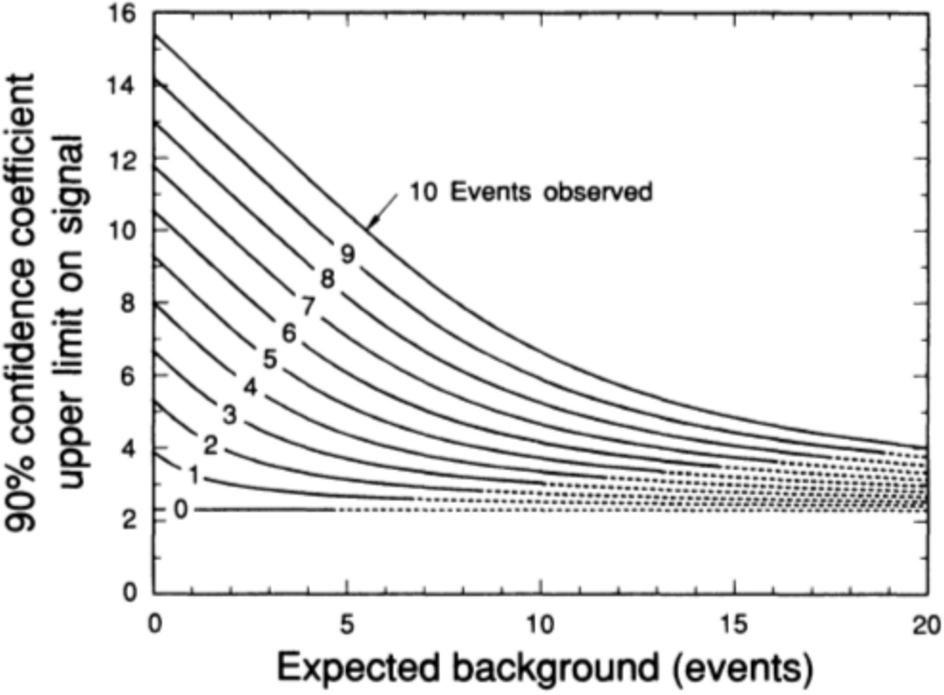
\includegraphics[width=.5\textwidth]{Appendix/limitEstimate}
	\caption{90\,\% CL upper limits as a function of the number of background events and the observation, from PhysRevD.45.S1.97
	\label{fig:limitEstimate}}
\end{center}
\end{figure}
